\documentclass[10pt, twocolumn]{article}

%%%%%%%%%%%%%%%%%%%%%%%%%%%%%%%%%%%%%%%%%%%%%%%%%%%%%%%%%%%%%%%%%%%%%%%%%%%%%%%
%%%% Cover page
\title{MECH 351: Thermodynamics II}
\date{\today}
\author{Anthony Bourboujas}

\makeatletter
\let\Title\@title
\let\Author\@author
\let\Date\@date
\makeatother

%%%%%%%%%%%%%%%%%%%%%%%%%%%%%%%%%%%%%%%%%%%%%%%%%%%%%%%%%%%%%%%%%%%%%%%%%%%%%%%
%%%% Preamble
%%%%%%%%%%%%%%%%%%%%%%%%%%%%%%%%%%%%%%%%%%%%%%%%%%%%%%%%%%%%%%%%%%%%%%%%%%%%%%%
%%%% Packages
\usepackage[utf8x]{inputenc} % Accept different input encodings
\usepackage[T1]{fontenc} % Standard package for selecting font encodings
\usepackage{lmodern} % Font name; classic: lmodern
\usepackage[english]{babel} % Multilingual support for LaTeX
% \usepackage{abstract} % Control the typesetting of the abstract environment
\usepackage{amsmath} % AMS mathematical facilities for LaTeX
\usepackage{amssymb} % TeX fonts from the American Mathematical Society
\usepackage{amsthm} % Typesetting theorems (AMS style)
\usepackage{array} % Extending the array and tabular environments
% \usepackage[backend=biber,style=ieee,sorting=none]{biblatex}
\usepackage{bold-extra} % Use bold small caps and typewriter fonts
\usepackage{cellspace} % Ensure minimal spacing for table cells
\usepackage{chemformula} % Command for typesetting chemical formulas and reactions
% \usepackage{colortbl} % Add colour to LaTeX tables
\usepackage{comment} % Selectively include/exclude portions of text
\usepackage{csquotes} % Context sensitive quotation facilities
% \usepackage[en-US,showdow]{datetime2} % Formats for dates, times and time zones
% \usepackage{diagbox} % Table heads with diagonal lines
\usepackage{enumitem} % Control layout of itemize, enumerate, description
\usepackage{esint} % Extended set of integrals for Computer Modern
\usepackage{graphicx} % Enhanced support for graphics
% \usepackage{listings} % Typeset source code listings using LaTeX
% \usepackage{lipsum} % Easy access to the Lorem Ipsum dummy text
\usepackage{mathrsfs} % Support for using RSFS fonts in maths
% \usepackage{matlab-prettifier} % Pretty-print Matlab source code
\usepackage{moreverb} % Extended verbatim
\usepackage{multicol} % Intermix single and multiple columns
\usepackage{multirow} % Create tabular cells spanning multiple rows
% \usepackage{pgfplots} % Plots
% \usepackage{pgfplotstable} % Loads, rounds, format and post-processes numerical tables (generates table from CSV)
% \usepackage{pdfpages} % Include PDF document in LaTeX
% \usepackage{rotating} % Rotation tools, including rotated full-page floats with sidewaysfigure
\usepackage[scr]{rsfso} % A mathematical calligraphic font based on rsfs
\usepackage{setspace} % Set space between lines
\usepackage{soul} % Hyphenation for letterspacing, underlining, and more
\usepackage{threeparttable} % Tables with captions and notes all the same width
% \usepackage{verbatim} % Reimplementation of and extensions to LaTeX verbatim
\usepackage{wrapfig} % Produces figures which text can flow around
\usepackage{xcolor} % Driver-independent color extensions for LaTeX
\usepackage{xurl} % Verbatim with URL-sensitive line breaks, allow URL breaks at any alphanumerical character

%%%%%%%%%%%%%%%%%%%%%%%%%%%%%%%%%%%%%%%%%%%%%%%%%%%%%%%%%%%%%%%%%%%%%%%%%%%%%%%
%%%% Lengths
% 1cm = 10mm = 28pt = 1/2.54in
% 1ex = height of a lowercase 'x' in the current font
% 1em = width of an uppercase 'M' in the current font

%%%% Spacing in math mode
% \!                         = -3/18em
% \,                         = 3/18em
% \:                         = 4/18em
% \;                         = 5/18em
% \ (space after backslash!) = space in normal text
% \quad                      = 1em
% \qquad                     = 2em

% \setlength{\baselineskip}{1em} % Vertical distance between lines in a paragraph
% \renewcommand{\baselinestretch}{1.0} % A factor multiplying \baslineskip
\setlength{\columnsep}{0.75cm} % Distance between columns
% \setlength{\columnwidth}{} % The width of a column
\setlength{\columnseprule}{1pt} % The width of the vertical ruler between columns
% \setlength{\evensidemargin}{} % Margin of even pages, commonly used in two-sided documents such as books
% \setlength{\linewidth}{} % Width of the line in the current environment.
% \setlength{\oddsidemargin}{} % Margin of odd pages, commonly used in two-sided documents such as books
% \setlength{\paperwidth}{} % Width of the page
% \setlength{\paperheight}{} % Height of the page
\setlength{\parindent}{0cm} % Paragraph indentation
\setlength{\parskip}{6pt} % Vertical space between paragraphs
% \setlength{\tabcolsep}{} % Separation between columns in a table (tabular environment)
% \setlength{\textheight}{} % Height of the text area in the page
% \setlength{\textwidth}{} % Width of the text area in the page
% \setlength{\topmargin}{} % Length of the top margin
\setlist{
  %%%% Vertical spacing
  topsep = 0pt,
  partopsep = 0pt,
  parsep = 0pt,
  itemsep = 0pt,
  %%%% Horizontal spacing
  leftmargin = 0.5cm,
  rightmargin = 0cm,
  % listparindent = 0cm,
  % labelwidth = 0cm,
  % labelsep = 0cm,
  % itemindent = 0cm
}
\addtolength{\cellspacetoplimit}{2pt}
\addtolength{\cellspacebottomlimit}{2pt}

%%%%%%%%%%%%%%%%%%%%%%%%%%%%%%%%%%%%%%%%%%%%%%%%%%%%%%%%%%%%%%%%%%%%%%%%%%%%%%%
%%%% Page layout
\usepackage{layout} % View the layout of a document
\usepackage{geometry} % Flexible and complete interface to document dimensions
% 1cm = 10mm = 28pt = 1/2.54in
% ex = height of a lowercase 'x' in the current font
% em = width of an uppercase 'M' in the current font
\geometry{
  a4paper,
  top         = 1cm,
  bottom      = 1cm,
  left        = 1.5cm,
  right       = 1.5cm,
  includehead = true,
  includefoot = true,
  landscape   = false, % Paper orientation
  twoside     = false,
}
% \geometry{showframe} % Show paper outline for the text area and page

%%%%%%%%%%%%%%%%%%%%%%%%%%%%%%%%%%%%%%%%%%%%%%%%%%%%%%%%%%%%%%%%%%%%%%%%%%%%%%%
%%%% Header and footer style
\usepackage{fancyhdr} % Extensive control of page headers and footers in LaTeX
\pagestyle{fancy}
% Options: \leftmark (chapter title), \rightmark(section title), \thepage (page number), \thechapter(chapter number), \thesection (section number)
\lhead{\thetitle}
\chead{}
\rhead{}
\lfoot{}
\cfoot{\thepage}
\rfoot{}

%%%%%%%%%%%%%%%%%%%%%%%%%%%%%%%%%%%%%%%%%%%%%%%%%%%%%%%%%%%%%%%%%%%%%%%%%%%%%%%
%%%% URL insertion settings
\usepackage{hyperref} % Extensive support for hypertext in LaTeX
\definecolor{black}{RGB}{0, 0, 0} % rgb(0, 0, 0)
\definecolor{blue}{RGB}{0, 0, 255} % rgb(0, 0, 255)
\hypersetup{
  % unicode            = true,
  pdftitle           = {\thetitle},
  pdfauthor          = {\theauthor},
  % pdfsubject       = {},
  %%%% Reference
  % bookmarks          = true,
  bookmarksnumbered  = true,
  bookmarksopen      = true, % Open the bookmarks
  bookmarksopenlevel = 2, % Open until 1 level (section)
  %%%% Bookmarks
  breaklinks         = true,
  pdfborder          = {0 0 0},
  % backref            = true, % Add links into bibliography
  % pagebackref        = true,
  % hyperindex         = true, % Add links into index
  %%%% Color
  colorlinks         = true,
  linkcolor          = black, % Internal links color
  citecolor          = black,
  urlcolor           = blue, % Hyperlinks color
  filecolor          = black,
}

\usepackage{varioref} % Intelligent page reference
\usepackage[capitalise,noabbrev]{cleveref}
\usepackage{prettyref} % Make label references "self-identity" with \prettyref{#1}
\newrefformat{cha}{chapter \textbf{\nameref{#1}} \vpageref{#1}} % {chapter \textbf{\nameref{#1}} on page \pageref{#1}}
\newrefformat{sec}{section \textbf{\nameref{#1}} \vpageref{#1}} % {section \textbf{\nameref{#1}} on page \pageref{#1}}
% \newrefformat{fig}{\vref{#1}} % {Figure \ref{#1} on page \pageref{#1}}
% \newrefformat{tab}{\vref{#1}} % {Table \ref{#1} on page \pageref{#1}}
% \newrefformat{eqn}{\vref{#1}}
% \newrefformat{lis}{\emph{\nameref{#1}} \vpageref{#1}}

%%%%%%%%%%%%%%%%%%%%%%%%%%%%%%%%%%%%%%%%%%%%%%%%%%%%%%%%%%%%%%%%%%%%%%%%%%%%%%%
%%%% Physics units settings
% Dependencies
\usepackage{booktabs} % Publication quality tables in LaTeX
\usepackage{caption} % Customizing captions in floating environments
\usepackage{helvet} % Load Helvetica, scaled
\usepackage{cancel} % Place lines through maths formulae

\usepackage{siunitx} % A comprehensive (SI) units package
\sisetup{
  exponent-product     = \cdot, % Symbol between number and power of ten
  group-minimum-digits = 5, % Number of digits when 3 digits separation appear
  % inter-unit-product   = \cdot, % Symbol between units (when several units are used)
  output-complex-root  = \ensuremath{i}, % How i math should be seen
  % prefixes-as-symbols  = false, % Translate prefixes (kilo, centi, milli, micro,...) into a power of ten
  separate-uncertainty = true, % Write uncertainty with +-
  scientific-notation  = engineering,
}

%%%%%%%%%%%%%%%%%%%%%%%%%%%%%%%%%%%%%%%%%%%%%%%%%%%%%%%%%%%%%%%%%%%%%%%%%%%%%%%
%%%% Theorems and proofs
\numberwithin{equation}{section}
% \makeatletter
% \g@addto@macro\th@remark{\thm@headpunct{:}}
% \makeatother
\theoremstyle{remark}
\newtheorem*{example}{Example}
\newtheorem*{remark}{Remark}

%%%%%%%%%%%%%%%%%%%%%%%%%%%%%%%%%%%%%%%%%%%%%%%%%%%%%%%%%%%%%%%%%%%%%%%%%%%%%%%
%%%% User-defined environments
% Remove the space before the enumerate and itemize environments
\let\oldenumerate\enumerate % Keep a copy of \enumerate (or \begin{enumerate})
\let\endoldenumerate\endenumerate % Keep a copy of \endenumerate (or \end{enumerate})
\renewenvironment{enumerate}{
  \begin{oldenumerate}
    \vspace{-6pt}
    }{
  \end{oldenumerate}
}

\let\olditemize\itemize % Keep a copy of \itemize (or \begin{itemize})
\let\endolditemize\enditemize % Keep a copy of \enditemize (or \end{itemize})
\renewenvironment{itemize}{
  \begin{olditemize}
    \vspace{-6pt}
    }{
  \end{olditemize}
}

\let\olddescription\description % Keep a copy of \description (or \begin{description})
\let\endolddescription\enddescription % Keep a copy of \enddescription (or \end{description})
\renewenvironment{description}{
  \begin{olddescription}
    \vspace{-6pt}
    }{
  \end{olddescription}
}

%%%%%%%%%%%%%%%%%%%%%%%%%%%%%%%%%%%%%%%%%%%%%%%%%%%%%%%%%%%%%%%%%%%%%%%%%%%%%%%
%%%% User-defined commands
\newcommand{\Romannumeral}[1]{\MakeUppercase{\romannumeral #1}} % Capital roman numbers
% \newcommand{\gui}[1]{\og #1 \fg{}} % French quotation marks
\renewcommand{\thefootnote}{[\arabic{footnote}]}

%%% Figure command
%% Include SVG files
\newcommand{\executeiffilenewer}[3]{
  \ifnum\pdfstrcmp{\pdffilemoddate{#1}}
    {\pdffilemoddate{#2}}>0
    {\immediate\write18{#3}}\fi
}
\newcommand{\includesvg}[1]{
  \executeiffilenewer{#1.svg}{#1.pdf}
  {
    % Inkscape must be installed in PATH and the user must include '--shell-escape' in the build arguments
    inkscape #1.svg --export-type=pdf --export-latex
  }
  \input{#1.pdf_tex}
}

%%% Math commands
%% Tables (requires cellspace package)
\newcolumntype{L}{>{\(\displaystyle}Cl<{\)}} % Column type for left-aligned math column
\newcolumntype{D}{>{\(\displaystyle}Cc<{\)}} % Column type for centered math column

%% Functions
\newcommand{\constant}{\mathrm{constant}} % Constant
\newcommand{\abs}[1]{\left| #1 \right|} % Absolute function
\newcommand{\erf}[1]{\mathrm{erf} \left( #1 \right)} % Error function
\newcommand{\erfc}[1]{\mathrm{erfc} \left( #1 \right)} % Complementary error function
\newcommand{\unitstep}[1]{\,\mathcal{U}\left( #1 \right)} % Unit step function
\newcommand{\diracdelta}[2]{\,\delta_{#1}\left( #2 \right)} % Dirac delta function


%% Derivatives and integrals
\newcommand{\diff}[2]{\mathrm{d}^{#1} #2} % Letter 'd' of differentials
\newcommand{\diffint}[1]{\,\diff{}{#1}} % Differential with a space for integrals
\newcommand{\derivative}[2]{\frac{\diff{}{#1}}{\diff{}{#2}}} % Derivative
\newcommand{\nderivative}[3]{\frac{\diff{#1}{#2}}{\diff{}{#3^{#1}}}} % Derivative of degree n
\newcommand{\partialderivative}[2]{\frac{\partial #1}{\partial #2}} % Partial derivative
\newcommand{\npartialderivative}[3]{\frac{\partial^{#1} #2}{\partial #3^{#1}}} % Partial derivative of degree n
\newcommand{\direcderivative}[2]{D_{\vec{#1}}\,#2} % Directional derivative

\newcommand{\Laplace}[1]{\mathcal{L}\left\{ #1 \right\}} % Laplace transform notation
\newcommand{\invLaplace}[1]{\mathcal{L}^{-1}\left\{ #1 \right\}} % Inverse Laplace transform notation

%% Set
\newcommand{\set}[3]{\mathbb{#1}_{#2}^{#3}} % Set of numbers
\newcommand{\integerset}{\mathbb{Z}} % Set of integer numbers (compatibility)
\newcommand{\realset}{\mathbb{R}} % Set of real numbers (compatibility)

%% Limits
\newcommand{\limit}[3]{\lim_{#1 \to #2}{#3}} % Limit from a point to another
\newcommand{\rlimit}[3]{\lim_{#1 \to #2^{+}}{#3}} % Right limit from a point to another
\newcommand{\llimit}[3]{\lim_{#1 \to #2^{-}}{#3}} % Left imit from a point to another
\newcommand{\modulus}[1]{\,\left[ #1 \right]} % Modulus notation

%% Vectors
\newcommand{\ivec}{\hat{\mathrm{i}}} % i vector
\newcommand{\jvec}{\hat{\mathrm{j}}} % j vector
\newcommand{\kvec}{\hat{\mathrm{k}}} % k vector
\renewcommand{\Vec}[1]{\overrightarrow{#1}} % Vector notation for expression with more than one letter
\newcommand{\norm}[1]{\left\| #1 \right\|} % Norm notation for expression with just one letter
\newcommand{\normvec}[1]{\left\| \vec{#1} \right\|} % Norm notation for expression with just one letter
\newcommand{\Normvec}[1]{\left\| \Vec{#1} \right\|} % Norm notation for expression with more than one letter
\newcommand{\comp}[2]{\mathrm{comp}_{\vec{#2}}\vec{#1}} % Components
\newcommand{\proj}[2]{\mathrm{proj}_{\vec{#2}}\vec{#1}}
\newcommand{\grad}[1]{\vec{\nabla}#1} % Gradient notation
\newcommand{\frames}[2]{\left( #1 \right)_{#2}} % Frame definition

\newcommand{\curl}[1]{\mathrm{curl}\,\vec{#1}} % Curl of a vector field
\newcommand{\divergence}[1]{\mathrm{div}\,\vec{#1}} % Divergence of a vector field


%%%%%%%%%%%%%%%%%%%%%%%%%%%%%%%%%%%%%%%%%%%%%%%%%%%%%%%%%%%%%%%%%%%%%%%%%%%%%%%
%%%% Beginning of the document
\begin{document}
\maketitle % Insert the cover page
% \tableofcontents
% \layout % Show a drawing of page layout
% \renewcommand{\abstractname}{} % Change the abstract title

First Law equation for a closed system:
\begin{equation} \tag{1} \label{eq:First-Law-closed-system}
  \begin{split}
    \Delta E_{1 \rightarrow 2} & = Q_{1 \rightarrow 2} - W_{1 \rightarrow 2}                                                                                \\
    & = \Delta E_{\mathrm{kinetic},1 \rightarrow 2} + \Delta E_{\mathrm{potential},1 \rightarrow 2} + \Delta U_{1 \rightarrow 2}
  \end{split}
\end{equation}

First Law equation for an open system:
\begin{multline} \tag{2} \label{eq:First-Law-open-system}
  \dot{E}_{CV} = \dot{Q}_\mathrm{in} - \dot{W}_\mathrm{out}
  + \sum_\mathrm{in}{\dot{m}_\mathrm{in}\left( \frac{1}{2}v_\mathrm{in}^2 + gz_\mathrm{in} + h_\mathrm{in} \right)} \\
  - \sum_\mathrm{out}{\dot{m}_\mathrm{out}\left( \frac{1}{2}v_\mathrm{out}^2 + gz_\mathrm{out} + h_\mathrm{out} \right)}
\end{multline}



\section{Rankine cycle}
Assumptions:
\begin{itemize}
  \item Steady flow, \(\Delta \dot{m} = 0\)
  \item Pumps and turbines are isentropic, \(\Delta s_\mathrm{pumps} = \Delta s_\mathrm{turbines} = 0\)
  \item Boilers and condensers are isobaric, \(\Delta P_\mathrm{boilers} = \Delta P_\mathrm{condensers} = 0\)
  \item No pressure losses in the cycle
  \item Temperature at the inlet and outlet of a closed regenerator are equal
  \item Kinetic and potential energy are negligible, \(\Delta E_\mathrm{kinetic} = \Delta E_\mathrm{potential} = 0\)
  \item Expansion valve is isenthalpic
\end{itemize}


\subsection{Simple Rankine cycle}
The Rankine cycle is a steam power cycle that operates with both liquid and gas states.
Processes of a simple Rankine cycle:
\begin{description}
  \item[\(1 \rightarrow 2\)] Compression in a pump from saturated liquid to compressed liquid
  \item[\(2 \rightarrow 3\)] Heating from compressed liquid to superheated gas
  \item[\(3 \rightarrow 4\)] Expansion in a turbine
  \item[\(4 \rightarrow 1\)] Cooling from gas to saturated liquid
\end{description}

For a compressed liquid at a temperature \(T\) and a pressure \(P\), if \(P \ll P_\mathrm{table}\):
\begin{align*}
  u_\mathrm{liq}   & \approx u_f (T)              \\
  \nu_\mathrm{liq} & \approx \nu_f (T)            \\
  s_\mathrm{liq}   & \approx s_f (T)              \\
  h_\mathrm{liq}   & \approx u_f (T) + P\nu_f (T)
\end{align*}

For an incompressible liquid, the work of a pump can be approximated to \(w_{1 \to 2} = \nu(P_1 - P_2 )\)

Efficiency of a simple Rankine cycle:
\[
  \begin{split}
    \eta_\mathrm{thermal} & = \frac{\dot{W}_\mathrm{net}}{\dot{Q}_\mathrm{in}} = \frac{w_{1 \to 2} + w_{3 \to 4}}{q_{2 \to 3}} \\
    & = \frac{h_1 - h_2 + h_3 - h_4 }{h_3 - h_2 }
  \end{split}
\]

\subsection{Improve the Rankine cycle}
\subsubsection{Simple Rankine cycle}
To improve the efficiency of a simple Rankine cycle, there are several approaches, each with some operational constraints:
\begin{itemize}
  \item \(T_1 \searrow\)
        \begin{olditemize}
          \item absolute limit of ground temperature
          \item more leaks in
          \item lower turbine flow quality
        \end{olditemize}
  \item \(T_3 \nearrow\)
        \begin{olditemize}
          \item temperature of the hot source based on application
          \item \(T_3\) too high could weaken the blade of the turbine
        \end{olditemize}
  \item \(P_2 \nearrow\)
        \begin{olditemize}
          \item increase in \(T_3\)
          \item more stress on the boiler
        \end{olditemize}
\end{itemize}


\subsubsection{Reheat Rankine cycle}
A reheat Rankine cycle uses several turbines between which the fluid is reheated.
\begin{figure*}[ht] % Position: b (bottom), t (top), h (here), ! (insist)
  \centering
  \caption{Ideal reheat Rankine cycle}
  \label{fig:ideal-reheat-Rankine}
  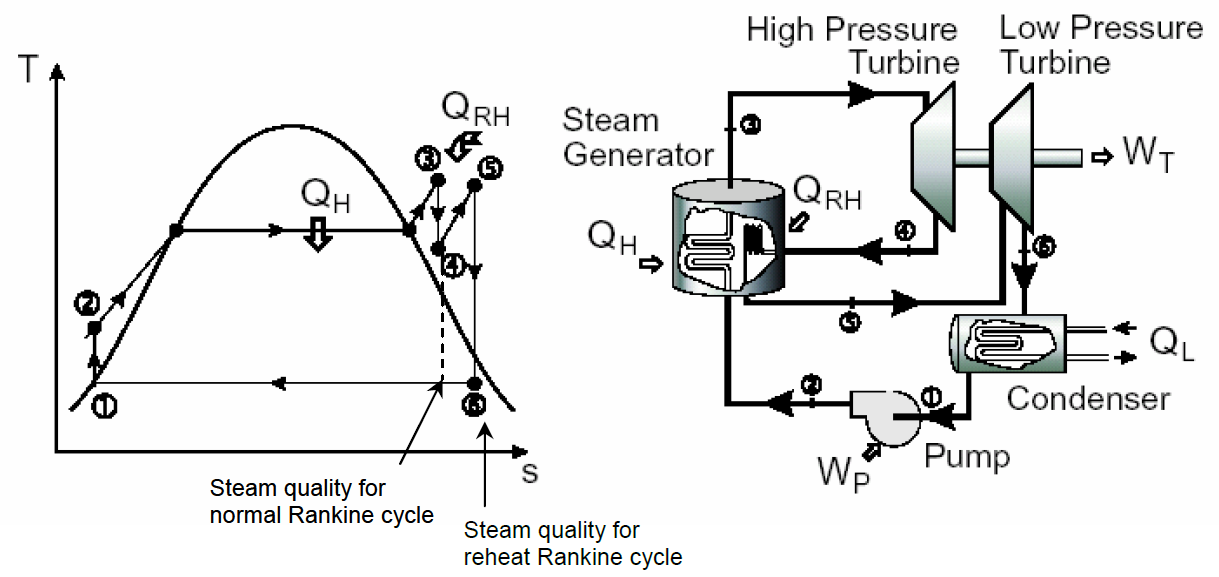
\includegraphics[width = 0.9\linewidth]{../../images/mech/mech-351/ideal-reheat-Rankine-cycle.png}
\end{figure*}


\subsubsection{Regeneration Rankine cycle}
A regeneration Rankine cycle uses a feed water heater: the hot fluid from the outlet of the turbine exchange heat with the cold fluid from the outlet for the pump.
This can be done with two types of feed water heater:
\begin{description}
  \item[Open feed water heater:] the fluid from the pump and the turbine are mixed together, so there is a need of another pump before the boiler to raise the pressure.
  \item[Closed feed water heater:] the fluid from the pump and the turbine are not mixed together, thus only one pump is needed for the cycle.
        Also, it is the most thermodynamically efficient as using a counter flow, the heating process is almost done at constant temperature, meaning it is almost a reversible process.
\end{description}

\begin{figure*}[ht] % Position: b (bottom), t (top), h (here), ! (insist)
  \centering
  \caption{Ideal regeneration Rankine cycle with an open feed water heater}
  \label{fig:ideal-rgeneration-Rankine-OFWH}
  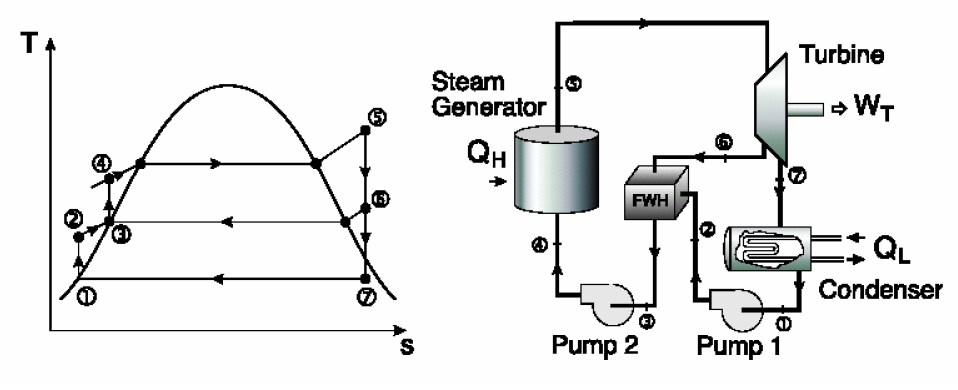
\includegraphics[width = 0.9\linewidth]{../../images/mech/mech-351/ideal-regeneration-Rankine-cycle-OFWH.png}
\end{figure*}

In order to have the most efficient cycle, we should have the inlet of the pumps as a saturated liquid with a pressure of \(P_\text{OFWH} \approx \sqrt{P_\mathrm{boiler} P_\mathrm{condenser}}\)

\subsubsection{Cogeneration Rankine cycle}
The cogeneration Rankine cycle uses the steam from the outlet of the turbine to heat something else called a process heater (e.g. heat a building, a house, etc).
Since it can exceed Carnot efficiency \(\mu_\mathrm{Carnot}\), the efficiency of the cogeneration cycle is called the utilization factor \(\varepsilon_u\) :
\[
  \varepsilon_u = \frac{\dot{W}_\mathrm{net} + \dot{Q}_\text{process heater}}{\dot{Q}_\mathrm{in}}
\]

The cogeneration is very useful as at times of high demand for process heat, all the steam in redirected in the process heater, while at time of high demand for power, all the steam goes to the turbine.


\subsection{Problem solving steps to find the efficiency}
\begin{enumerate}
  \item Draw cycle with all its components (pumps, boilers, turbines, condensers, feed water heaters, traps and process heaters)
  \item Write the assumptions
  \item Draw the T-s diagram
  \item Build the table of states with the following thermodynamic variables:
        \begin{olditemize}
          \item Mass flow rate \(\dot{m}\) [\(\si{\kilogram\per\second}\)] (do not forget split fractions \(y_i\))
          \item Temperature \(T\) [\(\si{\celsius}\)]
          \item Pressure \(P\) [\(\si{\pascal}\)]
          \item Specific entropy \(s\) [\(\si{\joule\per\kilogram\per\kelvin}\)]
          \item Specific enthalpy \(h\) [\(\si{\joule\per\kilogram}\)]
          \item Specific volume [\(\si{\metre\cubed\per\kilogram}\)]
        \end{olditemize}
  \item \label{itm:Rankine-efficiency-formula} Find the efficiency formula for this Rankine cycle (do not forget that at splitters, mass flow rate \(\dot{m}\) might be in term of split fractions \(y_i\))
  \item Study each components (transition between states)
        \begin{oldenumerate}
          \item Write the First Law equation for an open system \eqref{eq:First-Law-open-system}
          \item Simplify the First Law equation using the assumptions
          \item Find either the specific heat exchange \(q\), specific work \(w\), split fraction \(y_i\), or specific enthalpy \(h\)
        \end{oldenumerate}
  \item Repeat previous step until finding every unknown of the efficiency formula found at step \ref{itm:Rankine-efficiency-formula}
  \item Compute the efficiency
\end{enumerate}


\section{Brayton cycle}
Assumptions:
\begin{itemize}
  \item Steady flow, \(\Delta \dot{m} = 0\)
  \item Air standard approximation (air everywhere, combustion replaced with equivalent external heat input)
  \item Ideal gas, \(P \nu = RT\)
  \item Compressors and turbines are isentropic, \(\Delta s_\mathrm{compressors} = \Delta s_\mathrm{turbines} = 0\)
  \item Boilers and condensers are isobaric, \(\Delta P_\mathrm{boilers} = \Delta P_\mathrm{condensers} = 0\)
  \item No pressure losses in the cycle
  \item Temperature at the inlet and outlet of a closed regenerator are equal
  \item Pressure ratio constant in the cycle, \(r_P = \frac{P_2}{P_1} = \frac{P_3}{P_4}\)
  \item Specific pressure heat is constant, \(\Delta C_P = 0 \implies H_{1 \to 2} = m C_P (T_2 - T_1)\)
  \item Kinetic and potential energy are negligible, \(\Delta E_\mathrm{kinetic} = \Delta E_\mathrm{potential} = 0\)
  \item Expansion valve is isenthalpic
\end{itemize}


\subsection{Simple Brayton cycle}
The Brayton cycle is a gas power cycle that operates only in gas states.
Processes of a simple Brayton cycle:
\begin{description}
  \item[\(1 \rightarrow 2\)] Compression in a pump
  \item[\(2 \rightarrow 3\)] Combustion using fuel
  \item[\(3 \rightarrow 4\)] Expansion in a turbine
\end{description}
In a real Brayton cycle, the air is taken from the outside at state 1 and exhausted back outside at state 4 along with the combustion products.

Processes of a simple Brayton cycle with air standard approximation:
\begin{description}
  \item[\(1 \rightarrow 2\)] Compression in a pump
  \item[\(2 \rightarrow 3\)] Heating
  \item[\(3 \rightarrow 4\)] Expansion in a turbine
  \item[\(4 \rightarrow 1\)] Cooling
\end{description}

Relations for an ideal gas in an isentropic process:
\begin{gather}\label{eq:ideal-gas-isentropic-process}
  P_1{\nu_1}^k = P_2{\nu_2}^k                                                                                 \\
  \frac{T_2}{T_1} = \left( \frac{P_2}{P_1} \right)^{\frac{k - 1}{k}} = \left( \frac{V_1}{V_2} \right)^{k - 1} \nonumber\\
  C_P = \frac{kR}{k - 1} \text{ and } C_V = \frac{R}{k - 1} \nonumber
\end{gather}

Efficiency of a simple Brayton cycle:
\[
  \eta_\mathrm{thermal} = \frac{\dot{W}_\mathrm{net}}{\dot{Q}_\mathrm{in}} = 1 - \frac{T_1}{T_2} = 1 - \frac{1}{{r_P }^{\frac{k - 1}{k}}}
\]
where \(r_P = \frac{P_2}{P_1} = \frac{P_3}{P_4}\) is the pressure ratio of the cycle and \(k= \frac{C_P}{C_V}\) is the isentropic constant.

The work of the pump in a Brayton cycle is not negligible compared to a Rankine cycle, thus the back-work ratio quantify the percentage of the turbine power that is used by the compressor:
\[
  r_{BW} = \abs{\frac{\dot{W}_\mathrm{compressor}}{\dot{W}_\mathrm{turbine}}}
\]



\subsection{Improve the Brayton cycle}
\subsubsection{Simple Brayton cycle}
Since the efficiency depends directly on the pressure ration \(r_P\), the efficiency can be improved by increasing the pressure ratio.
This can be done only to a certain extent as too much pressure leads to very high temperatures which could melt the turbine blades.


\subsubsection{Regeneration Brayton cycle}
A regeneration Brayton cycle uses a regenerator: the hot air from the outlet of the turbine exchange heat with the cold air from the outlet for the pump.
This can be done with closed regenerator: the air from the pump and the turbine are not mixed together.

When using an ideal regenerator, the efficiency of a Brayton cycle is:
\[
  \eta_\mathrm{thermal} = 1 - r_{BW}
\]


\subsubsection{Reheat Brayton cycle}
A reheat Brayton cycle uses several turbines between which the air is reheated.


\subsubsection{Intercooling Brayton cycle}
An inter-cooling Brayton cycle uses several compressors between which the air is cooled.


\subsection{Problem solving steps to find the efficiency}
\begin{enumerate}
  \item Draw cycle with all its components (compressors, combustion chambers, turbines, condensers, regenerators)
  \item Write the assumptions
  \item Draw the T-s diagram
  \item Build the table of states with the following thermodynamic variables:
        \begin{olditemize}
          \item Pressure \(P\) [\(\si{\pascal}\)]
          \item Temperature \(T\) [\(\si{\celsius}\)]
          \item Temperature \(T\) [\(\si{\kelvin}\)]
        \end{olditemize}
  \item \label{itm:Brayton-efficiency-formula} Find the efficiency formula for this Brayton cycle
  \item Study each components (transition between states)
        \begin{oldenumerate}
          \item Write the First Law equation for an open system \eqref{eq:First-Law-open-system}
          \item Simplify the First Law equation using the assumptions
          \item Write the isentropic relations \eqref{eq:ideal-gas-isentropic-process}
          \item Find either the specific heat exchange \(q\), specific work \(w\), temperature \(T\) or pressure \(P\)
        \end{oldenumerate}
  \item Repeat previous step until finding every unknown of the efficiency formula found at step \ref{itm:Brayton-efficiency-formula}
  \item Compute the efficiency
\end{enumerate}


\subsection{Jet engines}
Assumptions changed:
\begin{itemize}
  \item Kinetic and potential energy are negligible, \(\Delta E_\mathrm{kinetic} = \Delta E_\mathrm{potential} = 0\)
  \item Presence of a diffuser and a nozzle
  \item Pressure ratio no longer constant in the cycle, \(r_{P,\mathrm{turbine}} \neq r_{P,\mathrm{compressor}}\)
  \item Back-work ratio is 100\%, \(\abs{\dot{W}_\mathrm{compressor}} = \abs{\dot{W}_\mathrm{turbine}}\)
\end{itemize}

Thrust equation for generic propulsive device:
\[
  F_\mathrm{thrust} = (\dot{m}_\mathrm{air} + \dot{m}_\mathrm{fuel})v_\mathrm{out} + P_\mathrm{out}A_\mathrm{out} - \dot{m}_\mathrm{air}v_\mathrm{in} - P_\mathrm{in}A_\mathrm{in}
\]
Thrust equation for generic propulsive device (air standard approximation, constant area):
\[
  F_\mathrm{thrust} = \dot{m}_\mathrm{air} (v_\mathrm{out} - v_\mathrm{in}) + A_\mathrm{engine} (P_\mathrm{out} - P_\mathrm{in})
\]
Maximum thrust is at \(P_\mathrm{out} = P_\mathrm{in}\), meaning:
\[
  F_\mathrm{thrust} = \dot{m}_\mathrm{air} (v_\mathrm{out} - v_\mathrm{in})
\]

Propulsive efficiency of a jet engine cycle:
\[
  \eta_\mathrm{propulsive} = \frac{\dot{W}_\mathrm{propulsion}}{\dot{Q}_\mathrm{in}} = \frac{F_\mathrm{thrust} v_\mathrm{in}}{\dot{m}_\mathrm{fuel} Q_{HV}}
\]
where \(Q_{HV}\) is the heating value of the fuel.


\subsubsection{Problem solving steps to find the efficiency}

\begin{enumerate}
  \item Draw cycle with all its components (diffusers, compressors, combustion chambers, turbines, condensers, regenerators, nozzles)
  \item Write the assumptions
  \item Draw the T-s diagram
  \item Build the table of states with the following thermodynamic variables:
        \begin{olditemize}
          \item Pressure \(P\) [\(\si{\pascal}\)]
          \item Temperature \(T\) [\(\si{\celsius}\)]
          \item Temperature \(T\) [\(\si{\kelvin}\)]
          \item Velocity \(v\) [\(\si{\metre\per\second}\)]
        \end{olditemize}
  \item \label{itm:jet-engine-efficiency-formula} Write the efficiency and thrust formulas for this the jet engine cycle
  \item Study each components (transition between states)
        \begin{oldenumerate}
          \item Write the First Law equation for an open system \eqref{eq:First-Law-open-system}
          \item Simplify the First Law equation using the assumptions
          \item Write the isentropic relations \eqref{eq:ideal-gas-isentropic-process}
          \item Find either the specific heat exchange \(q\), specific work \(w\), temperature \(T\), pressure \(P\) or velocity \(v\)
        \end{oldenumerate}
  \item Repeat previous step until finding every unknown of the efficiency formula found at step \ref{itm:jet-engine-efficiency-formula}
  \item Compute the efficiency
\end{enumerate}


\section{Reciprocating devices (Otto, Diesel, Atkinson/Miller cycles)}
These cycles are working with a piston-cylinder device.
The processes are unsteady, meaning we have too use the First Law for a closed system \eqref{eq:First-Law-closed-system}.

Terms:
\begin{description}
  \item[TDC:] top dead center (piston at the top), minimum volume
  \item[BDC:] bottom dead center (piston at the bottom), maximum volume
  \item[\(V_D\):] displacement volume, \(V_D = \frac{\pi B^2}{4}L\) where \(B\) is the bore (cylinder radius) and \(L\) is the vertical displacement
  \item[\(V_C\):] clearance volume, \(V_C = V_\mathrm{TDC}\)
  \item[\(V_\mathrm{total}\):] total cylinder volume, \(V_\mathrm{total} = V_\mathrm{BDC} = V_D + V_C\)
  \item[\(r_C\):] compression ratio, \(r_C = \frac{V_\mathrm{BDC}}{V_\mathrm{TDC}} = \frac{\nu_\mathrm{BDC}}{\nu_\mathrm{TDC}}\)
\end{description}


Assumptions:
\begin{itemize}
  \item Closed system
  \item Air standard approximation (air everywhere, combustion replaced with equivalent external heat input)
  \item Ideal gas, \(P \nu = RT\)
  \item No pressure losses in the cycle
  \item Specific volume heat is constant, \(\Delta C_v = 0 \implies U_{1 \to 2} = m C_v (T_2 - T_1)\)
  \item Kinetic and potential energy are negligible, \(\Delta E_\mathrm{kinetic} = \Delta E_\mathrm{potential} = 0\)
\end{itemize}


\subsection{Otto cycle}
The Otto cycle is the cycle found in gasoline engine cars.
Processes of the Otto cycle:
\begin{description}
  \item[\(1 \rightarrow 2\)] Isentropic compression from the BDC to the TDC
  \item[\(2 \rightarrow 3\)] Isochoric heating
  \item[\(3 \rightarrow 4\)] Isentropic expansion from the TDC to the BDC (the work is done here)
  \item[\(4 \rightarrow 1\)] Isochoric cooling
\end{description}

Efficiency of an ideal Otto cycle:
\[
  \eta_\mathrm{thermal} = \frac{\dot{W}_\mathrm{net}}{\dot{Q}_\mathrm{in}} = 1 - \frac{T_1}{T_2} = 1 - \frac{1}{{r_C}^{k - 1}}
\]
where \(k= \frac{C_P}{C_V}\) is the isentropic constant.


Mean effective pressure (way to quantify the efficiency of an engine):
\[
  MEP = \frac{W_\mathrm{net}}{V_D} = \frac{w_\mathrm{net}}{\nu_\mathrm{BDC} - \nu_\mathrm{TDC}} = \frac{w_\mathrm{net}}{R\left(\frac{T_2}{P_2} - \frac{T_1}{P_1} \right)}
\]


\subsection{Otto vs Diesel vs Atkinson}
The Otto cycle has an isochoric heating, the Diesel cycle has an isobaric heating, and the Atkinson cycle is an improvement of the Otto cycle which re-use the excess of pressure at the end of the cycle.


\subsection{Diesel cycle}
Since the Diesel cycle only compress air, the compression ratio is higher than the Otto cycle because there is no risk of auto-ignition.
However, given the same compression ratio \(r_C\), the Otto cycle is more efficient because the Diesel cycle stays at the same pressure during the fuel combustion phase.

Cutoff ratio:
\[
  \beta = \frac{\nu_\mathrm{intermediate}}{\nu_\mathrm{minimum}} = \frac{\nu_3}{\nu_2}
\]
The cutoff ratio is used in determining the efficiency of the cycle and the pressure and temperature at the final state (usually state 4) since:
\begin{align*}
  \frac{P_4}{P_3} & = \left( \frac{\beta}{r_C} \right)^k       \\
  \frac{T_4}{T_3} & = \left( \frac{\beta}{r_C} \right)^{k - 1}
\end{align*}

Efficiency of an ideal Diesel cycle:
\[
  \eta_\mathrm{thermal} = \frac{\dot{W}_\mathrm{net}}{\dot{Q}_\mathrm{in}} = 1 - \frac{1}{{r_C}^{k - 1}} \left[ \frac{\beta^k - 1}{k (\beta - 1)} \right]
\]
where \(k= \frac{C_P}{C_V}\) is the isentropic constant.


\subsection{Problem solving steps to find the efficiency}
\begin{enumerate}
  \item State that the control volume is the gas in the piston-cylinder device
  \item Write the assumptions
  \item Draw the P-\(\nu\) and T-s diagrams according to the cycle
  \item Build the table of state with the following thermodynamic variables:
        \begin{olditemize}
          \item Pressure \(P\) [\(\si{\pascal}\)]
          \item Temperature \(T\) [\(\si{\celsius}\)]
          \item Temperature \(T\) [\(\si{\kelvin}\)]
          \item Specific volume \(\nu\) [\(\si{\metre\cubed\per\kilogram}\)]
        \end{olditemize}
  \item \label{itm:Reciprocating-efficiency-formula} Find the efficiency formula for this reciprocating device
  \item Study each transition between states
        \begin{oldenumerate}
          \item Write the First Law equation for a closed system \eqref{eq:First-Law-closed-system}
          \item Simplify the First Law equation using the assumptions
          \item Write the isentropic relations \eqref{eq:ideal-gas-isentropic-process}
          \item Find either the specific heat exchange \(q\), specific work \(w\), temperature \(T\), pressure \(P\) or cutoff ration \(\beta\)
        \end{oldenumerate}
  \item Repeat previous step until finding every unknown of the efficiency formula found at step \ref{itm:Reciprocating-efficiency-formula}
  \item Compute the efficiency
\end{enumerate}


\section{Refrigeration}
Assumptions:
\begin{itemize}
  \item Steady flow, \(\Delta \dot{m} = 0\)
  \item Compressors are isentropic, \(\Delta s_\mathrm{compressors} = 0\)
  \item Evaporators and condensers are isobaric, \(\Delta P_\mathrm{evaporators} = \Delta P_\mathrm{condensers} = 0\)
  \item No pressure losses in the cycle
  \item Kinetic and potential energy are negligible, \(\Delta E_\mathrm{kinetic} = \Delta E_\mathrm{potential} = 0\)
  \item Expansion valve is isenthalpic
\end{itemize}


\subsection{Simple vapor-refrigeration cycle}
The refrigeration cycle is very similar to a Rankine cycle:
\begin{description}
  \item[\(1 \rightarrow 2\)] Compression in a compressor from saturated gas to superheated gas
  \item[\(2 \rightarrow 3\)] Cooling from superheated gas to saturated liquid
  \item[\(3 \rightarrow 4\)] Expansion in an expansion valve
  \item[\(4 \rightarrow 1\)] Heating from mixed phase to saturated gas
\end{description}

\begin{figure*}[ht] % Position: b (bottom), t (top), h (here), ! (insist)
  \centering
  \caption{Ideal vapor-refrigeration cycle}
  \label{fig:ideal-vapor-refrigeration}
  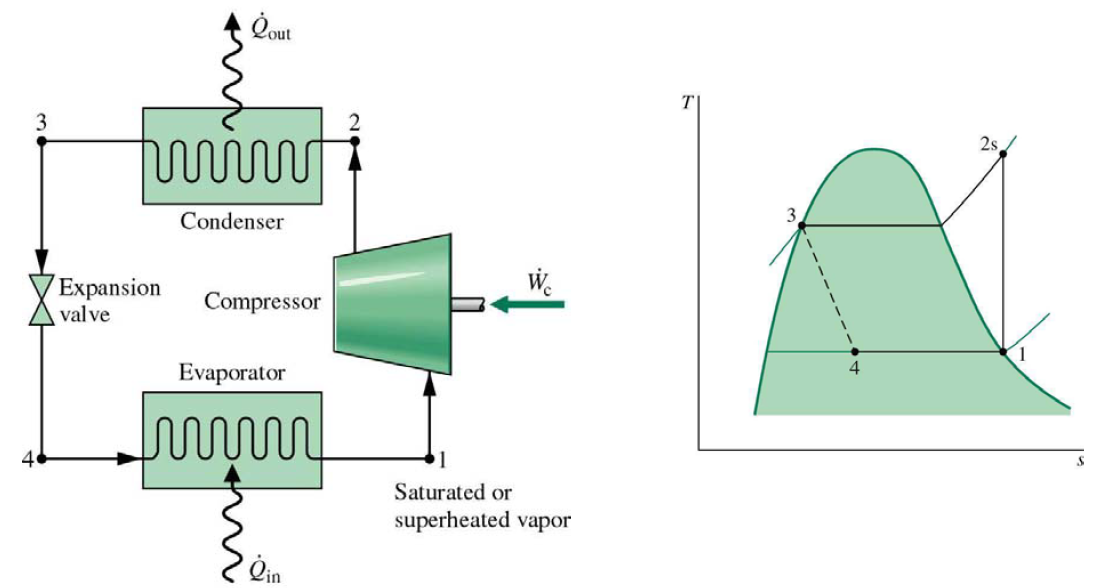
\includegraphics[width = 0.9\linewidth]{../../images/mech/mech-351/ideal-vapor-refrigeration-cycle.png}
\end{figure*}

The refrigeration cycle has an other advantages: by looking at the heat rejection side, the refrigeration becomes a heat pump.


To quantify a refrigeration cycle and a heat pump, the coefficient of performance is used:
\begin{align*}
  \mathrm{COP}_\mathrm{ref} & = \beta_\mathrm{ref} = \frac{\dot{Q}_\mathrm{in}}{\dot{W}_\mathrm{in}}                                                                                \\
  \mathrm{COP}_\mathrm{HP}  & = \beta_\mathrm{HP} = \frac{\dot{Q}_\mathrm{out}}{\dot{W}_\mathrm{in}} = 1 + \frac{\dot{Q}_\mathrm{in}}{\dot{W}_\mathrm{in}} = 1 + \beta_\mathrm{ref}
\end{align*}

\subsection{Improve the vapor-refrigeration cycle}
\subsubsection{Multi-stage refrigeration}
The multi-stage refrigeration cycle has multiple refrigeration cycle in it:

\begin{figure*}[ht] % Position: b (bottom), t (top), h (here), ! (insist)
  \centering
  \caption{Ideal two-stage refrigeration cycle}
  \label{fig:ideal-two-stage-refrigeration}
  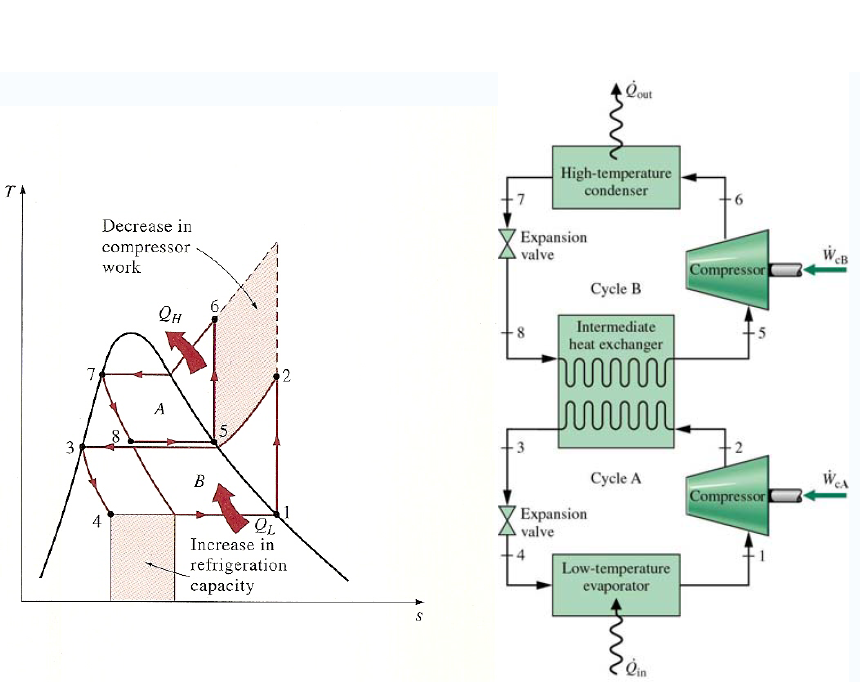
\includegraphics[width = 0.9\linewidth]{../../images/mech/mech-351/ideal-2-stage-refrigeration-cycle.png}
\end{figure*}


\subsubsection{Ground power source heat pump}
Since the coefficient of performance becomes low when the too much difference in temperature between the hot side and the cold side, one solution is to place the evaporator (or condenser if used as a heat pump) deep in the ground, where the temperature does not vary much during the year.
This way the difference of temperature between the two side remains fairly constant throughout the year, letting us have a constant coefficient of performance.


\subsection{Problem solving steps to find the efficiency}
\begin{enumerate}
  \item Draw cycle with all its components (compressors, evaporators, condensers, heat exchanger and expansion valve)
  \item Write the assumptions
  \item Draw the T-s diagram
  \item Build the table of states with the following thermodynamic variables:
        \begin{olditemize}
          \item Mass flow rate \(\dot{m}\) [\(\si{\kilogram\per\second}\)] (do not forget split fractions \(y_i\))
          \item Temperature \(T\) [\(\si{\celsius}\)]
          \item Pressure \(P\) [\(\si{\pascal}\)]
          \item Specific entropy \(s\) [\(\si{\joule\per\kilogram\per\kelvin}\)]
          \item Specific enthalpy \(h\) [\(\si{\joule\per\kilogram}\)]
          \item Specific volume [\(\si{\metre\cubed\per\kilogram}\)]
        \end{olditemize}
  \item \label{itm:refrigeration-COP-formula} Find the coefficient of performance formula for this refrigeration cycle (do not forget that the mass flow rate \(\dot{m}\) might be different in each loop)
  \item Study each components (transition between states)
        \begin{oldenumerate}
          \item Write the First Law equation for an open system \eqref{eq:First-Law-open-system}
          \item Simplify the First Law equation using the assumptions
          \item Find either the specific heat exchange \(q\), specific work \(w\), mass flow rate \(\dot{m}\) or specific enthalpy \(h\)
        \end{oldenumerate}
  \item Repeat previous step until finding every unknown of the coefficient of performance formula found at step \ref{itm:refrigeration-COP-formula}
  \item Compute the coefficient of performance
\end{enumerate}


\section{Mixtures}
A mixture is a collection of different substances together.
It is not the same a multiphase (liquid and gas phase commonly referred as a mixture) as a multiphase is only composed of one substance.

\begin{example}
  Air is a mixture: 79\% \ch{N2} + 21\% \ch{O2} in mole.
\end{example}

In this class, we will only deal with ideal mixtures.
% #TODO: add what an ideal mixture is

For ideal mixtures, every extensive variables add up:
\begin{align*}
  m_\mathrm{mix} & = m_A + m_B + \cdots = \sum{m_i} \\
  n_\mathrm{mix} & = n_A + n_B + \cdots = \sum{n_i}
\end{align*}
\[
  \begin{array}{|l}
    m_i [\si{\kilogram}] \text{: mass of component } i \\
    n_i [\si{\mole}] \text{: number of mole of component } i
  \end{array}
\]

We can define two properties using the mass and the number of mole:
\begin{description}
  \item[Mass fraction:] \(x_i = \frac{m_i}{m_\mathrm{mix}} \implies \sum{x_i} = 1\)
  \item[Mole fraction:] \(y_i = \frac{n_i}{n_\mathrm{mix}} \implies \sum{y_i} = 1\)
  \item[Molar mass of a mixture:] \(M_\mathrm{mix} = \frac{m_\mathrm{mix}}{n_\mathrm{mix}} = \sum{y_i M_i}\)
\end{description}
The composition of a mixture is completely defined by either the set of \(\{x_i\}\) or the set of \(\{y_i\}\).

\begin{example}
  Air defined by 79\% \ch{N2} + 21\% \ch{O2} in mole.
  \begin{align*}
    M_\mathrm{air}          & = 0.79 \times 2 \times 14 + 0.21 \times 2 \times 16                         \\
                            & = \SI{28.84e-3}{\kilogram\per\mole}                                         \\
    \implies R_\mathrm{air} & = \frac{R}{M_\mathrm{air}} \approx \SI{288}{\joule\per\kilogram\per\kelvin}
  \end{align*}
  where \(R = \SI{8.3145}{\joule\per\mole\per\kelvin}\).
\end{example}

\begin{example}
  Air defined by 79\% \ch{N2} + 20\% \ch{O2} + 1\% \ch{CO2} in mole.
  \begin{align*}
    M_\mathrm{air}          & = \SI{28.96e-3}{\kilogram\per\mole}                                         \\
    \implies R_\mathrm{air} & = \frac{R}{M_\mathrm{air}} \approx \SI{287}{\joule\per\kilogram\per\kelvin}
  \end{align*}
  where \(R = \SI{8.3145}{\joule\per\mole\per\kelvin}\).
\end{example}

Mass fraction in term of molar fraction and vice-versa:
\begin{align*}
  x_i = \frac{y_i M_i}{\sum{y_k M_k}} &  & y_i = \frac{\frac{x_i}{M_i}}{\sum{\frac{x_k}{M_k}}}
\end{align*}

\begin{example}
  Air defined by 79\% \ch{N2} + 21\% \ch{O2} in mole.
  \[
    \begin{array}{c|c|c|c|c}
              & y_i  & M_i & m_i (\SI{1}{\mole}) & x_i   \\ \hline\hline
      \ch{N2} & 0.79 & 28  & 6.72                & 0.233 \\
      \ch{O2} & 0.21 & 32  & 22.12               & 0.767 \\ \hline
              &      &     & 28.84               & 1
    \end{array}
  \]
\end{example}

\begin{example}
  Car exhaust defined by 70\% \ch{N2} + 22\% \ch{CO2} + 8\% \ch{H2O} in mass.
  \[
    \begin{array}{c|c|c|c|c}
               & x_i  & M_i & n_i (\SI{1}{\gram}) & y_i   \\ \hline\hline
      \ch{N2}  & 0.70 & 28  & 0.025               & 0.735 \\
      \ch{CO2} & 0.22 & 44  & 0.005               & 0.147 \\
      \ch{H2O} & 0.08 & 18  & 0.004               & 0.118 \\ \hline
               &      &     & 0.034               & 1
    \end{array}
  \]
\end{example}

Other extensive thermodynamic properties:
\begin{description}
  \item[Internal energy:] \(U_\mathrm{mix} = U_A + U_B + \cdots = \sum{U_i}\) and \(u_\mathrm{mix} = \sum{x_i u_i}\)
  \item[Enthalpy:] \(H_\mathrm{mix} = H_A + H_B + \cdots = \sum{H_i}\) and \(h_\mathrm{mix} = \sum{x_i h_i}\)
  \item[Entropy:] \(S_\mathrm{mix} = S_A + S_B + \cdots + S_\mathrm{mixing} = \sum{S_i} + S_\mathrm{mixing}\)
\end{description}

When dealing with mixtures, a state is defined using two independent intensive thermodynamic properties and \(n - 1\) extra properties of the mixture per degree of freedom, where \(n\) is the number of components.

Moreover, in order to solve problems, two closure conditions are needed, the first one being thermal equilibrium (\(T_\mathrm{mix} = T_A = T_B = \cdots = T_i\)) and the second one, a choice between:
\begin{description}
  \item[Dalton's law:] \(P_\mathrm{mix} = P_A + P_B + \cdots = \sum{P_i}\), which implies that \(V_\mathrm{mix} = V_A = V_B = \cdots = V_i\)
  \item[Amagat's law:] \(V_\mathrm{mix} = V_A + V_B + \cdots = \sum{V_i}\), which implies that \(P_\mathrm{mix} = P_A = P_B = \cdots = P_i\)
\end{description}


\subsection{Gas-vapor mixtures}
If we have a mixture of air and water vapor, here is the enthalpy of the mixture using Dalton's law:
\begin{align*}
  h_\mathrm{mix}      & = x_\mathrm{air} h_\mathrm{air}(T,P_\mathrm{air}) + x_\mathrm{\ch{H2O}} h_\mathrm{\ch{H2O}}(T,P_\mathrm{\ch{H2O}}) \\
  \iff H_\mathrm{mix} & = m_\mathrm{air} h_\mathrm{air}(T,P_\mathrm{air}) + m_\mathrm{\ch{H2O}} h_\mathrm{\ch{H2O}}(T,P_\mathrm{\ch{H2O}}) \\
  \iff h              & = h_\mathrm{air} + \omega h_\mathrm{\ch{H2O}}
\end{align*}
where \(\omega = \frac{m_\mathrm{\ch{H2O}}}{m_\mathrm{air}}\) is the specific humidity ratio and \(h\) is in \(\si{\joule}\mathrm{\ {\si{\kilogram}_{air}}^{-1}}\).


\subsubsection{Specific humidity ratio}
If we assume that both air and water vapor are ideal gases, the following relation for the specific humidity ratio \(\omega\) is obtained:
\[
  \omega = \frac{m_\mathrm{\ch{H2O}}}{m_\mathrm{air}} = \frac{M_\mathrm{\ch{H2O}}}{M_\mathrm{air}} \frac{P_\mathrm{\ch{H2O}}}{P - P_\mathrm{\ch{H2O}}} \approx 0.622 \frac{P_\mathrm{\ch{H2O}}}{P - P_\mathrm{\ch{H2O}}}
\]

% TODO: change kilogram of using SI{}{\kilogram\of{}}
The unit of the specific humidity ratio \(\omega\) is \(\mathrm{kg_{\ch{H2O}}\ {kg_{air}}^{-1}}\)

\begin{description}
  \item[Max \(\omega\):] at \(P_\mathrm{\ch{H2O}} = P_\mathrm{sat}(T)\) since the water vapor starts to condense and becomes liquid water, this state is called fully moist air
  \item[Min \(\omega\):] at \(P_\mathrm{\ch{H2O}} = 0\), this state is called fully dry air
\end{description}


\subsubsection{Relative humidity}
The relative humidity \(\phi\) has been defined since the specific humidity ratio \(\omega\) depends on the pressure \(P\) and the temperature \(T\), meaning the same value of \(\omega\) does not represent the same felt-humidity.
\begin{align*}
  \phi        & = \frac{P_\mathrm{\ch{H2O}}}{P_\mathrm{sat}(T)} = \frac{\omega P}{\left( \omega + \frac{M_\mathrm{\ch{H2O}}}{M_\mathrm{air}} \right)P_\mathrm{sat}(T)} \\
  \iff \phi   & \approx \frac{\omega P}{( \omega + 0.622 )P_\mathrm{sat}(T)}                                                                                           \\
  \iff \omega & \approx 0.622 \frac{\phi P_\mathrm{sat}(T)}{P - \phi P_\mathrm{sat}(T)}
\end{align*}


\subsubsection{Processes}
\paragraph{Adiabatic saturation process}
The adiabatic saturation process takes an amount of air in, circulates it over a liquid water reservoir long enough so that the air is fully moist when it exit.
This experiment is a way to measure the specific humidity ratio \(\omega\) and the relative humidity \(\phi\).
It leads to the equation:
\[
  \omega_1 = \frac{C_{P,\mathrm{air}} (T_2 - T_1) + \omega_2 \left[ h_g(T_2) - h_f(T_2) \right]}{h_g(T_1) - h_f(T_2)}
\]
where \(\omega_2 = \frac{P_\mathrm{sat}(T_2)}{P - P_\mathrm{sat}(T_2)}\), and \(T_1\), \(T_2\) and \(P\) can be measured.

In order to simplify the way to find the specific humidity ratio \(\omega\) and the relative humidity \(\phi\), the psychrometric chart is used (\url{http://www.flycarpet.net/en/PsyOnline}).

\paragraph{Heating}
Heating is a constant specific humidity ratio process (\(\Delta\omega = 0\)) and thus corresponds to a horizontal path to the right on the psychrometric chart.

This explains why houses feels dryer in the winter: heaters are heating the room, thus decreasing the relative humidity in the room.

\paragraph{Cooling}
Cooling is a constant specific humidity ratio process (\(\Delta\omega = 0\)), and thus corresponds to a horizontal path to the left on the psychrometric chart.

\paragraph{Cooling with dehumidification}
Cooling with dehumidification is a two step process:
\begin{enumerate}
  \item Constant \(\omega\) cooling until reaching a relative humidity \(\phi = 100\%\)
  \item Constant \(\phi\) cooling while water start to condensate
\end{enumerate}

\paragraph{Evaporative cooling}
Evaporative cooling is cooling while humidifying the air and is a constant enthalpy process (\(\Delta h = 0\)).

\paragraph{Mixing}
Mixing corresponds to the mix of two or more state of air, with different properties, to get another state.
\[
  \frac{\dot{m}_{\mathrm{air},2}}{\dot{m}_{\mathrm{air},1}} = \frac{h_3 - h_1}{h_2 - h_3} = \frac{\omega_3 - \omega_1}{\omega_2 - \omega_3}
\]

Those two equations can be used to solve mixing problems graphically as they represent straight lines on the psychrometric chart and ratio of lines between states.


\section{Combustion}
For combustion, we need to be aware that enthalpy at a temperature and pressure is with respect to a reference:
\[
  h(T) = h^0_f + C_P(T - 298)
\]
where \(h^0_f\) is the enthaply of formation, which is the amount of enthalpy needed for a substance to be in stable state at \(\SI{25}{\celsius}\) and 1 atm.

By definition:
\begin{description}
  \item[\ch{H}: ] stable in \ch{H2} \(\implies h^0_{f,\ch{H2}} = 0\)
  \item[\ch{O}: ] stable in \ch{O2} \(\implies h^0_{f,\ch{O2}} = 0\)
  \item[\ch{N}: ] stable in \ch{N2} \(\implies h^0_{f,\ch{N2}} = 0\)
  \item[\ch{C}: ] stable in \ch{C(s)} \(\implies h^0_{f,\ch{C(s)}} = 0\)
\end{description}

This is used in combustion problems because we are dealing with a reaction, meaning reactives react together by detaching their atoms and form products by attaching to other atoms.
This change of molecular composition requires energy, which comes from the enthalpy of formation.


\subsection{Combustion problems}
\paragraph{Heat of reaction}
Heat produced by a combustion in a isobaric and isothermal process:
\[
  \dot{Q}_\mathrm{out} = \dot{n}_k \left( \sum_\mathrm{reactives}{\nu_i \tilde{h}^0_{f,i}} - \sum_\mathrm{products}{\nu_i \tilde{h}^0_{f,i}} \right)
\]
\[
  \begin{array}{|l}
    \dot{n}_k [\si{\mole\per\second}] \text{: mole flow rate of a substance } k \text{ of the reaction} \\
    \nu_i \text{: substance } i \text{ stoichiometric factor related to the substance } k               \\
    \tilde{h}^0_f [\si{\joule\per\mole}] \text{: enthalpy of formation}
  \end{array}
\]

\paragraph{Adiabatic flame temperature}
Let us find the products temperature via an isobaric and adiabatic combustion:
\begin{multline}
  0 = \sum_\mathrm{reactives}{\nu_i \left[ \tilde{h}^0_{f,i} + \tilde{C}_{P,i}(T_1 - 298) \right]} \\
  - \sum_\mathrm{products}{\nu_i \left[ \tilde{h}^0_{f,i} + \tilde{C}_{P,i}(T_2 - 298) \right]}
\end{multline}
\[
  \begin{array}{|l}
    \nu \text{: stoichiometric factor}                                        \\
    \tilde{h}^0_f [\si{\joule\per\mole}] \text{: enthalpy of formation}       \\
    \tilde{C}_P [\si{\joule\per\mole\kelvin}] \text{: specific pressure heat} \\
    T [\si{\kelvin}] \text{: temperature}
  \end{array}
\]
where \(T_2\) is the adiabatic flame temperature.

\paragraph{Constant volume explosion}
Combustion at a constant volume:
\[
  \begin{split}
    \Delta E & = \Delta U \\
    \iff U_1 & = U_2 \\
    \iff H_1 - P_1 V & = H_2 - P_2V \\
    \iff H_2 - H_1 & = V(P_2 - P_1) \\
  \end{split}
\]

\end{document}